\documentclass{article}
\usepackage{graphicx}
\usepackage[]{mdframed}
\usepackage{tabularx}
\usepackage{subfig}
\usepackage{placeins}
\usepackage{float}

\graphicspath{ {./images/} }
\usepackage[a4paper, total={6in, 8in}]{geometry}


\author{Sidharth Babu, SNB2593 \and Tianda Huang, TH32684}
\title{ECE 361E: Homework 3}

\begin{document}
\begin{mdframed}
    \maketitle
\end{mdframed}
\pagebreak

\section*{Problem 1}
\subsection*{Question 2}
\begin{tabularx}{\textwidth} { 
    | >{\centering\arraybackslash}X 
    | >{\centering\arraybackslash}X 
    | >{\centering\arraybackslash}X
    | >{\centering\arraybackslash}X
    | >{\centering\arraybackslash}X
    | >{\centering\arraybackslash}X
    | >{\centering\arraybackslash}X 
    | }
    \hline
    Model & Training Accuracy(\%) & Test Accuracy (\%) & Total time for training (s) & Number of Trainable Params & Floating Point Operations & GPU memory during training (mb)\\
    \hline
    VGG11 & 97.57 & 76.48 & 3011.79 & 9,750,922 & 306587648 & 1215 \\
    \hline
    VGG16 & 97.86 & 78.89 & 3622.42 & 14,655,050 & 551954432 & 1425 \\
    \hline
\end{tabularx}

\subsection*{Question 3}
\begin{figure}[h]
    \centering
    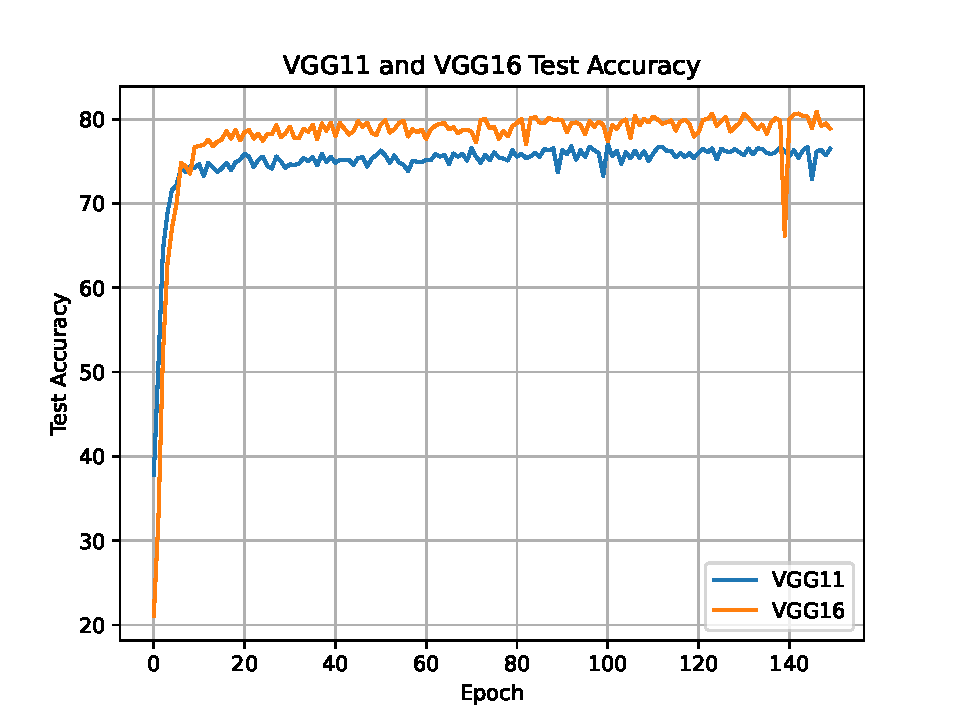
\includegraphics[width=0.5\textwidth]{graphing/vgg11_16_acc.pdf}
    \caption{Test Accuracy of VGG11 and VGG16}
    \label{fig:accuracy}
\end{figure}

VGG16 performs incrementally better than VGG11 on both train and test. However it has 1.5x the amount of trainable parameters and 1.8x the amount of floating point operations. 
The small accuracy boost is not worth the increase in computational complexity, and therefore we would choose VGG11 to train. 

\section*{Problem 2}
\subsection*{Question 2}
\begin{center}
\begin{tabular}{|*{7}{c|}}
    \hline
      & \multicolumn{2}{c|}{Total Inference Time [s]}  & \multicolumn{2}{c|}{RAM memory [MB]} & \multicolumn{2}{c|}{Accuracy[\%]} \\
    \cline{1-7}
      & MC1 & RaspberryPi & MC1 & RaspberryPi & MC1 & RaspberryPi \\
    \hline
    VGG11 & 658.23 & 680.61 & 380 & 146 & 76.48 & 76.48\\
    \hline
    VGG16 & 990.92 & 1172.01 & 338 & 174 & 78.89 & 78.89\\
    \hline
\end{tabular}
\end{center}

\subsection*{Question 3}
\section*{Problem 3}


\end{document}